\newcommand{\geomQuery}[4] {
  \begin{figure}[H]
    \centering
    \includesvg{../images/#2}{width=#3\textwidth}
    \caption[Explanation of the \textit{#1} geometry query]{\textbf{#1:}#4}
    \label{fig:#1}
  \end{figure}
}

\newcommand{\vecdatatype}[2]{
  \null
  \textbf{#1}
  \begin{adjustwidth}{1em}{0pt}
    #2
  \end{adjustwidth}
  \null
}

\newcommand{\codecallout}[2] {
  \null
  \begin{adjustwidth}{1em}{0pt}
    \textbf{#1:}
    #2
  \end{adjustwidth}
  \null
}


\renewcommand{\thefootnote}{\fnsymbol{footnote}}


\chapter{Background}\label{ch:background}

\section{Monte Carlo Geometry Queries}\label{sec:mc-geom-queries}

A Monte Carlo geometry kernel must provide robust support for the geometry
queries shown in Figures \ref{fig:Point Containment} -
\ref{fig:Measure}.

\geomQuery{Point Containment}{plc_query}{0.5}{
Given a set of volumes and particle location, $\mathbf{x}$, determine if the
point is inside, outside, or on the boundary of a volume.
}

\geomQuery{Next Surface}{dtb_query}{0.3}{
Given a volume, $\mathbf{V}$, particle location, $\mathbf{x}$, and particle
trajectory, \boldmath$\Omega$, determine the next surface, \boldmath$S$, of the
volume that the particle intersects with along \boldmath$\Omega$ and the
distance, \boldmath$d$ to that intersection.
}

\geomQuery{Closest Surface}{ctl_query}{0.3}{
Given a volume, \boldmath$V$, and particle location, \boldmath$x$, determine
the distance, \boldmath$d$, to to the nearest surface, \boldmath$S$, of the
volume in any direction.
}

\geomQuery{Next Volume}{next_vol_query}{0.5}{
Given a particle in volume, \boldmath$V_1$, and crossing a surface, \boldmath$S$,
determine the correct adjacent volume, \boldmath$V_2$.
}

\geomQuery{Surface Normal}{normal_query}{0.3}{
Given a surface, \boldmath$S$ and particle location, \boldmath$x$ determine
the normal vector, \boldmath$\vec{n}$, of the surface where the particle
crossing occurs.}

\geomQuery{Measure}{measure_query}{0.3}{
Given a volume, \boldmath$V$, or surface, \boldmath$S$ in the geometry,
determine properties of that entity such as the volume or area.
}

Failure to accurately satisfy geometry queries or calculate geometric values can
result in biased simulation results. Once such failure mode is lost particles
during simulation. Lost particles occur when the geometry kernel cannot
determine the particle's logical position, or which cell/volume contains the
particle, based on it's numerical position. Lost particles remove statistical
information from the simulation, and may influence results if particles are not
uniformly lost throughout phase space. Inaccurate measurement of volume or
surface area can result in incorrect values derived from simulation results,
such as surface current density tallies or k-effective values in criticality
simulations.

\section{Analytic Geometry Representations}\label{sec:analytic_geometry}

This section contains a discussion of common analytic geometry  representations
which are often used as native representations of Monte Carlo geometry.

\subsection{Implicit Surfaces}\label{subsec:implicit_surfaces}

An implicit surface is a multivariate function defined over an $ R^3 $ domain
onto the one-dimensional space, $ R $:

\begin{equation}
    \Omega(R^3)\rightarrow R
\end{equation}

These geometric representations are a rich and versatile representation of
closed manifolds used for modeling, simulation, and rendering. Implicit surfaces
are defined using the isocontour of a scalar function defined over all space -
unlike an \textit{explicit} representation of a surface which defines the subset
of space which the boundary occupies. Intuitively it might seem wasteful for a
definition to be true for all space considering the relatively small amount of
space the object will occupy, however a number of powerful tools for geometric
modeling using these representations will be discussed in this section.

An isocontour of this function with the value, $v$, can be described as:

\begin{equation}
  \Omega(\vec{x}) - v  = 0
\end{equation}

For simplicity, the boundary of an implicit surface is conventionally defined as
the isocontour for which $v=0$. As a result, any point inside of the surface
will have a negative value while any point outside of the surface will have a
positive value.

Unlike their explicit counterparts, implicit representations allow complex
topologies of surfaces to be integrated into a single representation. This is in
part because the function is defined for all space, allowing them to naturally
represent the merging and separation of disparate volumes. These properties
allow for straightforward representation of dynamic surfaces such as fluids,
though this is not yet of concern in the area of radiation transport. In
practice, implicit surfaces are often used to re-sample the model into some
other proxy for the geometry or render models via ray tracing. Additionally,
implicit surfaces can be used to generate triangle meshes for rasterization or
rendering on GPUs \cite{Sethian_1996} and can also be constructed from arbitrary
triangle meshes or point clouds \cite{Sigg_2006}. Implicit surfaces are
well-suited to these applications due to the integrated geometric properties
that can be quickly recovered from their analytic forms.

Geometric information needed for visualization and simulation can be
readily recovered from implicit surface representations. For example, a common
operation in particle transport is the determination of its containment by a
volume in the model. A quick evaluation of the implicit function for this point
will indicate its containment by the sign of the function.
%% Such a process is more complex in the case of an explicit or discretized
%% representation. Typically this involves casting a ray through the model and
%% counting up the intersections or relying on the orientation of triangle normals
%% to indicate an entering or exiting intersection. The oddness or eveness of the
%% number of crossings will then determine the points containment.
Additionally, the distance to nearest intersection with the surface from any
point in space can quickly be determined via the definition of a signed distance
function which is formally defined as:

\begin{align} \label{eq:sdf}
  & d(\vec{x}) = min(|\vec{x} - \vec{x_{I}}|) \\
  & \Omega(\vec{x})  \,s.t.  \, |\Omega(\vec{x})| = d(\vec{x})
\end{align}

\begin{align}
  d \, &- \, distance \, function \\
  \vec{x}_{I} \, &- \,surface \, interface
\end{align}

\noindent

\setcounter{footnote}{1}
These forms of implicit surface functions can be modified or selected such that the following
conditions are met:\footnote{The sign convention shown here is opposed to the
  sign convention commonly used for interior and exterior points in space. This
  sign convention is arbitrary and has been reversed for clarity in radiation
  transport where physical phenomena are simulated in the interior of objects
  rather than the space between them in rendering applications.}

\begin{figure}[H]
  \begin{center}
      \begin{itemize}
      \item $ \Omega(\vec{x}) = d(\vec{x}) = 0 $ for all $x$ on the surface boundary
      \item $ \Omega(\vec{x}) = d(\vec{x}) $ for all $x$ inside the surface boundary
      \item $ \Omega(\vec{x}) = -d(\vec{x}) $ for all $x$ outside the surface boundary
      \end{itemize}
  \end{center}
\end{figure}

Implicit surfaces are often used in time-dependent simulations due to their
natural extension into a fourth dimension ($ \Omega(\vec{x},t) - v  = 0 $) and
in turn their support for moving boundaries and changing topologies. Dynamic
geometries are not yet of concern for CAD-based Monte Carlo work, but
specialized forms of implicit surfaces are used as native geometry
representations in most Monte Carlo simulation codes.

\subsection{Constructive Solid Geometry}\label{subsec:csg}

Native Monte Carlo geometries are commonly formed from a standard set of
well-behaved implicit surfaces known as general quadratics. Constructive Solid
Geometry (CSG) representations combine these surfaces using Boolean operations to
form more complex objects as shown in Figure \ref{fig:csg_ex}.

\begin{figure}[h]
  \centering
  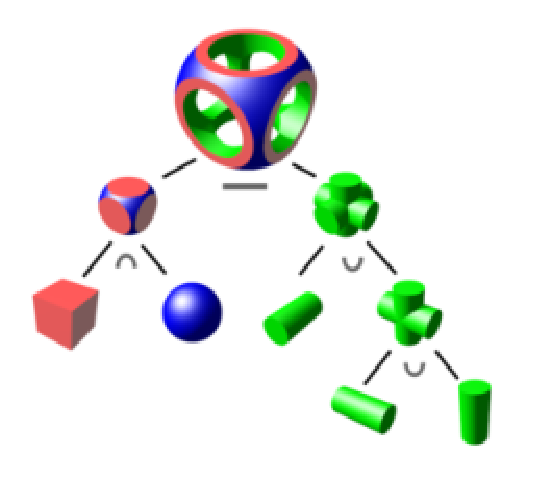
\includegraphics{csg_ex.eps}
  \caption[Example of CSG Boolean operations.]{An example of how CSG volumes are created using Boolean combinations
    of objects. The union of the three orthogonal cylinders is
    subtracted from the intersection of the box and sphere on the left to form
    the final volume at the top of the figure.}
  \label{fig:csg_ex}
\end{figure}

It is possible to construct complex geometries using CSG, but, as mentioned in
Chapter \ref{ch:introduction}, the interface for this work is typically
text-based. This format makes defining complex volumes a tedious and
time-consuming task. Detecting problems with the geometry definition is
straightforward for the same reason that particles can be robustly tracked
through the analytic description of the surfaces. Fixing
undefined regions of the geometry or detecting invalid volume definitions is
more difficult however.

The detection of intersections and particle containment queries in CSG
geometries is computationally inexpensive for volume definitions constructed
from a small number of surfaces, but, due to the logical combinations of
surfaces used to create volumes, the number of evaluations necessary to satisfy
these queries is linear with the number of surfaces in the definition. For
sufficiently large and complex models, it is not uncommon for volumes with many
surfaces to be artificially separated by planes to create multiple volumes with
fewer surfaces in their definition.

Visualization of CSG models is also somewhat limited. Because native formats for
CSG differ greatly between each Monte Carlo code, each typically provides its
own geometry visualization tools. These tools are commonly restricted to 2D
images of the model representing a user-specified slice through the
geometry.

% Other tools such as MCAM \cite{Liu_2005} and McCad
% \cite{Tsigetamirat_2008} allow for interactive visualization and repair of CSG
% models, but these systems often require simplifications of the true model in
% translation and limited export formats for various Monte Carlo codes.

\section{CAD Geometry}

Computer-Aided Design (CAD) systems allow for efficient and accurate
representation of geometrically complex domains. An example such a model is
shown in Figure \ref{fig:cad_fnsf}. Models can be created using interactive
visualization tools represented in 3D space with a rich tool set for volume and
surface creation. These creation and modification tools along with the immediate
visual verification of a user's work reduces human error in model generation and
design iteration.

\begin{figure}[H]
  \centering
  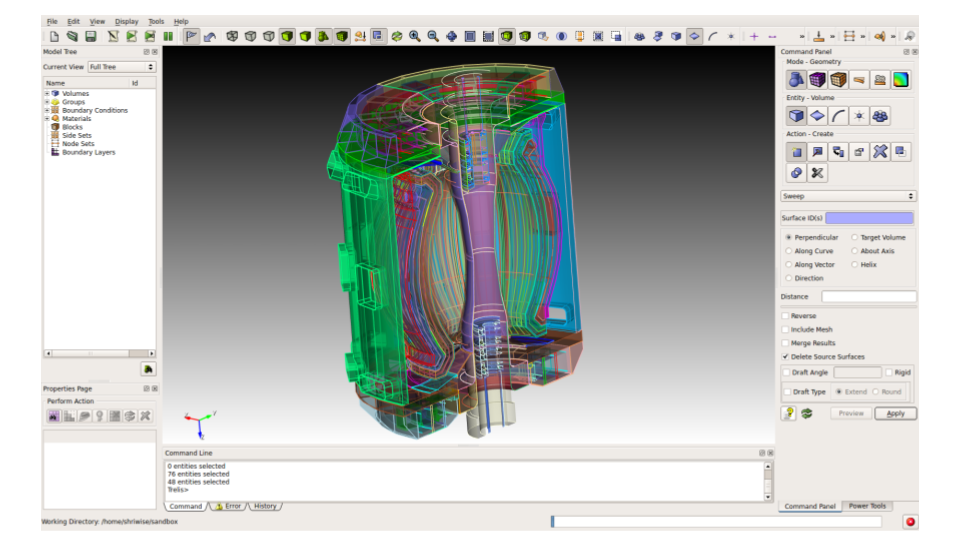
\includegraphics[scale=0.4]{cad_fnsf.png}
  \caption[CAD image of the FNSF facility.]{The Fusion Neutron Science Facility (FNSF)\cite{Kessel_2017} model
    displayed in the CUBIT geometry and mesh generation toolkit \cite{Blacker_1994}.}
  \label{fig:cad_fnsf}
\end{figure}

In addition to reducing human error and effort, CAD models provide a common
domain for analysis in other engineering domains such as fluid dynamics, heat
transfer, and structural engineering. This shared domain enables ease of
parametric studies and iterative design in coupled physics simulations. CAD
engines also provide the ability to represent free-form or higher-order
surfaces. The use of representations like splines, Bezier curves, and
subdivision surfaces allow for accurate representation of these arbitrarily
complex forms which would be impossible to accurately represent using CSG.

\section{CAD-Based Monte Carlo Radiation Transport}\label{sec:CAD-MCRT}

\subsection{Translation-Based Methods}

One approach to CAD-Based MCRT is to leverage the native geometry capabilities
of Monte Carlo codes by translating CAD geometries into CSG representations. In
this approach, the fidelity of the geometric representation is limited to the
geometric primitives available in the supported Monte Carlo code. Most codes
support only first and second order surfaces, so higher-order surfaces of the
CAD model must be approximated to accommodate the limited representation of the
native code. As a result, many of these methods will simplify single volumes
into smaller, less complex volumes able to be represented in CSG. This can be
problematic when tally information related to CAD entities is desired - surface
or volumetric fluxes for a single entity in the CAD model must now be mapped to
several entities in the CSG representation. The lack of one-to-one correlation
between CAD and CSG entities makes model manipulation difficult in that a change
to the CAD model may result more or fewer CSG entities after translation, adding
difficulty to tracking tally mapping. Several translation approaches have been
developed oriented toward the Monte Carlo N-Particle (MCNP) input format
developed at Los Alamos National Laboratory \cite{LANL_MCNP5_VOLIII}. A few of
these tools are described below:

\codecallout{MCAM}{The Monte Carlo Automatic Modeling (MCAM) tool was developed
  at the Chinese Academy of Sciences \cite{Yu_2013}. It supports both CAD-to-CSG
  and CSG-to-CAD conversion, relying on the ACIS \cite{ACIS_2018} geometry
  engine. It is capable of fixing gaps and overlaps in models and supports
  geometry creation. Volumes are decomposed into simplified, convex volumes
  during CAD-to-CSG translation.}

\codecallout{McCad}{McCad was developed at the Karlsruhe Institute of Technology
  in Germany and supports both CAD-to-CSG and CSG-to-CAD model conversion,
  relying on the Open CASCADE modeling engine to do so \cite{Grobe_2013,
    Opencascade_2018}. Void spaces in the model are automatically filled in
  McCad. McCad also decomposes single volumes into multiple volumes with
  simplified CAD definitions.}

Though other translation-based methods exist, these tools were selected for
discussion based on usage in analysis and development efforts at the
time of this work.

\subsection{Direct Transport Methods}

In the direct approach to CAD-Based MCRT, geometric queries are performed
directly on the CAD geometry. Unlike translation-based approaches, physics codes
must be modified to direct geometric operations to the CAD-Based
interfaces. Some direct methods perform queries on analytic CAD representations
while others use discretized forms, but in either case no simplification of the
geometry is involved. Direct computation on CAD geometries tends to be slower
than using native geometry because particle tracking is more computationally
expensive on complicated surface representations. Several recent implementations
of direct methods are listed below:

\codecallout{SERPENT}{Serpent \cite{Leppanen_2015} provides CAD-based transport
  using a geometry represented by individual stereo-lithography (STL) files or a
  ABAQUS mesh \cite{ABAQUS_2018} generated using CUBIT \cite{Blacker_1994}. It
  is expected that the volumes in these files do not occupy the same space and
  that each file contains a single, closed volume of triangles. Geometries can
  also be defined using both CSG and STL representations in this format
  \cite{Talamo_2018}. The use of separate files to represent volumes
  independently in this system makes interchanging parts in a geometry
  straightforward, but ensuring that these parts do not have gaps or overlaps
  can be a difficult task for users.}

\codecallout{MCNP6}{MCNP6 \cite{Goorley_2016}, developed at Los Alamos National
  Laboratory, has added a native capability for transport on a volumetric mesh
  of unstructured tetrehedra. Thus a conformal mesh can be generated using a CAD
  model for transport in this mode to achieve good geometry fidelity. Generating
  a geometrically constrained volumetric mesh is difficult (and sometimes
  impossible) for arbitrary geometries, however. Non-conformal meshes can also
  be used where tetrahedra overlapping volume boundaries will contain a
  homogenized mixture of the materials in the mesh element, but the effects of
  this approximation are difficult to quantify and depend greatly on the
  importance of the materials homogenized and mesh element characteristics.}

\codecallout{DAGMC}{ The Direct Accelerated Geometry Monte Carlo (DAGMC)
  software toolkit enables MCRT directly on CAD geometries \cite{Tautges_2004}
  using surface tessellations to represent volume boundaries.  DAGMC was
  developed at the University of Wisconsin - Madison and has been coupled with
  many Monte Carlo codes including MCNP (see Table
  \ref{tab:dagmc_implementations}). DAGMC relies on CUBIT (and its commercial
  counterpart, Trelis\cite{Trelis_2018}) for model importing, cleaning, and
  tessellation. Surface meshses are stored in the Mesh Oriented dAtaBase (MOAB)
  \cite{Tautges_2009}, developed at Argonne National Laboratory. CUBIT and
  Trelis features are used to ensure volumes do not overlap before
  discretization, and preprocessing steps ensure models are topologically
  watertight before transport\cite{Smith_2010}.}

Though each of the above methods has its merits, the work of this thesis has
been implemented in DAGMC. DAGMC has demonstrated robust transport capability
on models of varying geometric complexity for a number of physics
applications. As mentioned above, it accomplishes this by discretizing CAD surfaces into sets of
triangles representing surface boundaries. Volumes are then defined by all sets
of triangles which represent bounding surfaces of a given volume. This surface
mesh and the geometric relationships between sets of mesh elements, also known
as Meshsets, are stored in MOAB. These relationships, which preserve the geometric topology,
are stored in a hierarchical structure within MOAB, relating volumes to their
surfaces, surfaces to curves, and curves to geometric vertices. For the purposes
of this work, only the relationship between volumes and surfaces are of
concern. A depiction of the relationship between Meshsets in DAGMC geometries
can be seen in Figure \ref{fig:dagmc_geom_example}.

\begin{sidewaysfigure}
  \centering
  \includesvg{../images/moab_geom_fig}{width=0.45\textwidth,valign=t}
  \includesvg{../images/mesh_based_topology}{width=0.5\textwidth,valign=t}
  \caption[The DAGMC data model in MOAB.]{Left: Partial representation of a discretized DAGMC geometry. Right:
    A representation of the mesh-based hierarchy used to maintain topological
    information about the CAD geometry in MOAB.}
  \label{fig:dagmc_geom_example}
\end{sidewaysfigure}

It is important that topological relationships of the geometry-based Meshsets
are maintained to accelerate certain geometric queries on the surface mesh. For
example, \textit{Next Volume} (see Figure \ref{fig:Next Volume}) queries are
accelerated by using these relationships to directly determine which volume a
particle is passing into upon crossing a surface. In CSG, a surface crossing can
require a series of point containment checks for each volume to update the
logical position of a particle in another volume. Other queries become more
complicated, however, due to the sheer number of triangles needed to properly
define volumes with detailed features.

\textit{Next Surface} and \textit{Closest Surface} (see Figures \ref{fig:Next
  Surface} and \ref{fig:Closest Surface}) geometry queries, for example, can be
computationally expensive for volumes often composed of hundreds of thousands or
even millions of triangles. A convenient way to conceptualize geometric queries
on triangulated surfaces or volumes is to consider an equivalent CSG
representation constructed using a planar surface in place of each triangle in
the DAGMC model. The structure imposed by the Boolean combinations used to
define such volumes require that each surface be checked for an intersection
with the particle trajectory, resulting in a somewhat naive search for the
nearest intersection. This intersection can then be used to
determine the location of surface crossings.

The problem of finding a surface intersection for a given particle location and
trajectory for a set of geometric primitives is a well-researched problem in
the field of ray tracing. In this field, data structures designed to accelerate
the location of the nearest ray intersection are used to render animations and
images in real time.

% Other tools such as MCAM \cite{Liu_2005} and McCad
% \cite{Tsigetamirat_2008} allow for interactive visualization and repair of CSG
% models, but these systems often require simplifications of the true model in
% translation and limited export formats for various Monte Carlo codes.

\section{Ray Tracing Acceleration Data Structures}

Acceleration data structures for ray tracing are designed to rapidly narrow the
search for an intersection in 3D virtual space given a starting position and
trajectory used to construct a ray. This is accomplished by partitioning the
space and associating geometric primitives, usually triangles, with that
bounding partition. A search is performed by checking for an intersection with
this bounding partition. If the ray does not intersect with the partition, then
the set of primitives contained within that partition can be removed from the
search. If the ray does intersect with the partition, then the set of associated
primitives must be checked for intersection. Because a single separation into
two spatial partitions is often insufficient to increase search efficiency, this
partitioning process is performed recursively. The result is a tree, or
hierarchy, in which partitions at the top of tree are associated other
partitions, known as child nodes, rather than primitives. Partitions at the
bottom of the tree are known as leaf nodes and are directly associated with
geometric primitives representing the geometric boundary.

The search for a ray intersection then becomes a traversal of the tree in which
the children of the root node are checked for intersection. If an intersection
is found with one or both of the nodes, then the corresponding child nodes are
checked for intersection as well. This process is repeated until leaf nodes are
reached at which point primitives are checked for intersection. A simplified
version of this method can be found in Algorithm \ref{alg:bvh_traversal}.

Any primitives underneath a node with which the ray does not intersect can
immediately be rejected as a possibility for a hit. This allows many primitives
to rapidly be removed from the search, limiting the number of primitive
intersection checks to a small number compared to checking each primitive
individually. This technique reduces the algorithmic complexity of the search
from a brute force, or linear $O(N_{primitives})$ , search to a logarithmic
$O(\, log(N_{primitives}))$ search.

\newpage

\begin{lstlisting}[language=Python,basicstyle=\tiny,caption={[A general spatial hierarchy traversal algorithm.]{General algorithm for spatial hierarchy traversal to return the nearest intersection along a ray.}},label={alg:bvh_traversal},captionpos=b]
  def intersect_ray(tree_root, ray):

      stack.append(tree_root)

      while not stack.empty():

          node = stack.pop()

          if is_leaf(node):
              primitives = get_node_primitives(node)

              for primitive in primitives:
                  d = primitive_intersect(primitive, ray)
                  if d < dist: dist = d

              continue

          if node_intersect(node, ray):
              children = get_node_children(node)

              stack.append(children)

  return dist
\end{lstlisting}

The remainder of this section reviews heuristics, bounding constructs, and data
structure relationships used in rendering and scientific simulation
today. Next, two splitting heuristics used to build these data structures, the Entity Ratio Heuristic (ERH) and
Surface Area Heuristic (SAH) are discussed. After that, several common spatial
hierarchies are described including the KD-Tree, Bounding Volume Hierarchy
(BVH), and the octree. The remainder of this chapter describes CPU architecture
characteristics which allow adaptations of these hierarchical data structures to
achieve improved performance. This description includes a commentary on the
relevance of specific design elements in these accelerations to MCRT.

\subsection{Splitting Heuristics}\label{sec:heuristics}

There are two critical components that go into the creation of spatial
partitions in ray tracing hierarchies. The first is the selection of a candidate
splitting plane which is used to separate entities into one partition or
another. The second is the evaluation of the ``cost'' of that split. This cost
is a purely relative measure used to compare candidate splits for selection of a
best split curing construction. Because there is no way to know exactly how
expensive or inexpensive the cost of a split will be for the particular
simulation at hand, heuristics are used to estimate this cost and determine the
optimal splitting plane using limited information about the local nodes in the
tree. More specifically, this information is typically limited to the number of
primitives being split, bounds of the parent partition, and bounds of the
candidate child partitions. Split costs are compared to the relative cost of
forming a leaf node as well. If the cost of all splits is larger than that of
the current node, then it is declared a leaf node and the build process
continues in other areas of the hierarchy.

A virtually infinite number of planes could be tested to find the optimal plane for
dividing the entities between the child bounding volumes, but even if one were to
encounter such a splitting plane, it can be difficult to identify the plane as
such without more knowledge about the final tree structure. As a result, a
limited set of planes is tested for the best split based on a set of assumptions
about the problem at hand and the heuristics being used to evaluate split
costs. The most common method for split plane candidates is median plane
splitting in which the current partition is split in half along each axes of the
current bounding volume. Splitting plane costs are then evaluated and the split
with the lowest cost is selected. Other methods for plane selection exist, but
will not be discussed here as this work is more focused on traversal performance.

Two heuristics will now be discussed - the Entity Ratio Heuristic (ERH) and the
Surface Area Heuristic (SAH). The ERH uses the resulting number of primitives in
each child node to determine the cost of a split. The philosophy behind this
heuristic is to maintain the expected $O(log(N_{primitives}))$ cost of a ray
traversal by ensuring that the number of primitives are split as evenly as possible from
parent to child node. A form of this heuristic is presented in Equation
\eqref{eq:ERH}. The ERH cost is unit-less and bounded by zero and one. This
heuristic provides a finite limit on the expected cost, and makes it possible to
set both an upper and lower bound as both an unacceptably high and a ``good enough''
cost, respectively.

\begin{figure}[H]
\begin{equation}
\label{eq:ERH}
 C = \frac{|P_{R}-P_{L}|}{(P_{R} + P_{L})}
\end{equation}
  \begin{align*}
    C - & \,final \, cost \, evaluation \\
    P_{L} - & \, primitives\, contained\, by\, the\, left\, child  \\
    P_{R} - & \, primitives\, contained\, by\, the\, right\, child \\
  \end{align*}
  \caption[Formulation of the entity ratio heuristic.]{An example of the ERH calculation for a binary hierarchy.}
  \label{fig:ERH}
\end{figure}

The SAH applies spatial information as well as division of primitives to the
cost evaluation. Its full form is found in Equation \eqref{eq:SAH}. The SAH uses
the surface area of candidate child partitions relative to the parent
partition's surface area as an approximation for the probability that the children
will be visited after the parent volume. This evaluation relies on the
assumption that rays in the problem are globally isotropic. The explicit form of
the surface area heuristic was introduced in 1987 by Goldsmith and Salmon
\cite{Goldsmith_1987} and later formalized by MacDonald and Booth in 1990
\cite{MacDonald_1990}.

\begin{figure}[H]
  \begin{equation}
    C =  C_{t} + \frac{SA_{L}}{SA_{P}}P_{L}C_{i} +  \frac{SA_{R}}{SA_{P}}P_{R}C_{i}
    \label{eq:SAH}
  \end{equation}
  \begin{align*}
    C_{t} - & \,cost\, of\, traversal\, to\, child\, nodes \\
    C_{i} - & \, cost\, of\, primitive\, intersection\, check\, \\
    SA_{L} - &  \,surface\, area\, of\, left\, child \\
    P_{L} - & \, primitives\, contained\, by\, the\, left\, child  \\
    SA_{R} - & \, surface\, area\, of\, right\, child \\
    P_{R} - & \, primitives\, contained\, by\, the\, right\, child \\
    SA_{P} - & \, parent\, node's \, surface \, area \\
  \end{align*}
  \caption[Formulation of the surface area heuristic.]{A form of the surface area heuristic for a binary tree.}
  \label{fig:SAH}
\end{figure}

For the general case, ERH has not proved to be as effective as the SAH
\cite{Bittner_2013}, but as
seen in Chapter \ref{ch:high_valence} it is a useful tool in correcting the
surface area heuristic for triangle mesh features of a specific type. This
scenario will be discussed further in Chapter \ref{ch:high_valence}.

\subsection{KD-Trees}
\label{subsec:kd-trees}
The KD-Tree or multidimensional binary search tree was originally developed as
an acceleration data structure for querying records in databases and has since
found use in other applications including speech recognition, global information
systems, and ray tracing \cite{Bentley_1975}. KD-Trees operate by using single
values to represent divisions in a dimension of the problem space. A different
dimension is split in each level of the tree, and the process is recursively
repeated until a sufficiently small number of records or entities exist within
the resulting partitions of a split, resulting in leaf nodes of the tree.

This data structure is also commonly applied to virtual 3D space for ray
intersection queries. A different dimension of space is split in each level of
the tree just as is done in the context of an arbitrary database with different
indices of data. The values used for separation of entities in the tree now
represent a coordinate of a plane in that dimension; entities are sorted to
either side of that plane to perform a split. First, the problem space is
divided evenly in the x dimension. The two child partitions are divided along
the y axis and the resulting children of this division are subdivided along the
z axis. Divisions are typically selected in such a way that the largest extent
of the current candidate is bisected.

It is possible that by doing this primitive entities are divided by the plane as
well. There are a couple of ways in which this problem is addressed. The first
is to simply reference any intersected primitives in both of the children. This
means that some primitives may be checked for intersection more than once, but
requires no changes to the original model. The other solution is to divide the
primitive entities using the partition plane.  This solution requires
alterations to the model which may be undesirable under certain conditions and
violates the description of the KD-Tree as a pure querying structure by altering
the model.

\begin{figure}[H]
  \centering
  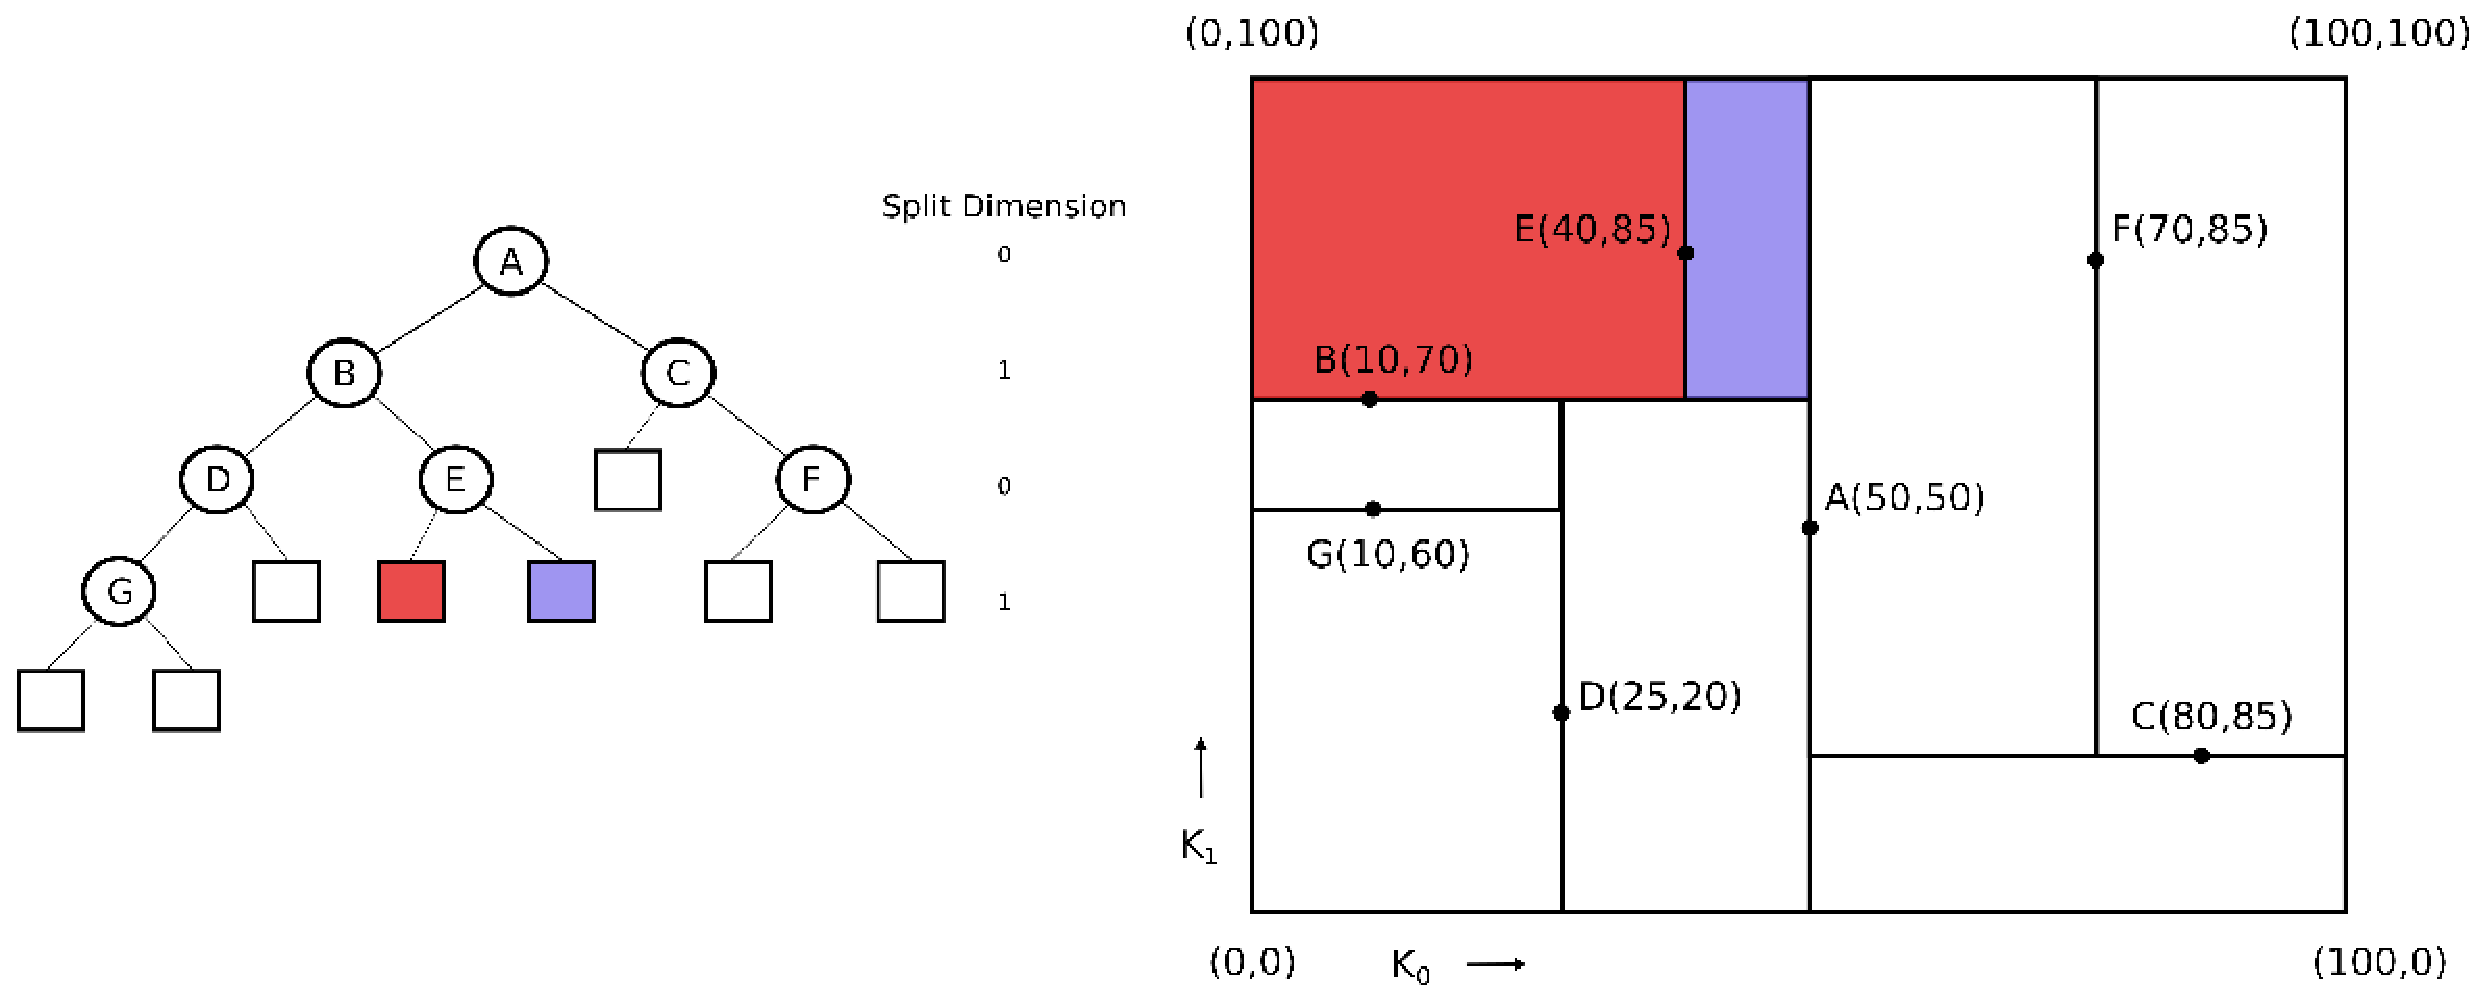
\includegraphics[scale=0.33]{2d_kd_eg.eps}
  \caption[A 2D KD-Tree example.]{Depiction of a two dimensional KD-Tree. Left: Graph representation of
    the KD-Tree with boxes representing leaf nodes. Right: Two dimensional space
    partitioned in the graph. Boxes represent the range of their respective
    sub-tree nodes. (Adapted from Bently et. al. \cite{Bentley_1975})}
  \label{fig:2D_kd_tree}
\end{figure}

KD-Trees are able to perform highly efficient spatial searches due to traversal
schemes developed based on the inherent characteristic of KD-Trees'
non-overlapping sibling nodes. As a KD-Tree is being constructed, an
ever-shrinking bounding box is being defined as one moves deeper into the
tree. At the leaves of a KD-Tree, a well-resolved bounding box can be
conceptualized using the coordinates of the last six splitting planes visited
and possibly the domain boundary. The conceptual construction of this box is one
way to move from node to node in a more efficient way than a more standard
depth-first approach shown in Algorithm \ref{alg:bvh_traversal}. The partitions
whose planes are used to construct this conceptual box can be linked to the
current partition in order to maintain a spatially localized search within the
hierarchy. These links are referred to as neighbor links and, as shown by Samet
et. al.\cite{Samet_1989}, can be used to significantly reduce traversal costs in
the KD-Tree. After a leaf is visited, neighbor links can be used to direct the
traversal to either the next adjacent leaf or a nearby interior node in the
tree, thus avoiding a depth-first style traversal in which the next step upon
visiting a leaf node is to return to the root node of the tree and continue. By
using these links to move directly to nearby leaf nodes, unnecessary shallow and
mid-level tree traversal steps can be avoided.

KD-Trees are frequently cited as being able to provide the best ray tracing
performance to date for certain geometries
\cite{Ernst_2007,Hurley_2002,Havran_2000}. In particular, KD-Trees are noted as
being better equipped to handle models with highly varying triangle
sizes/densities. In practice, KD-Trees also tend to be very deep, taking a long
time to construct, and can consume relatively high amounts of memory compared to
other acceleration data structures, however.

\subsection{Bounding Volume Hierarchies}%%Status: Done%%
\label{subsec:BVH}

A bounding volume hierarchy (BVH) uses a series of linked bounding volumes to
enclose sets of geometric primitives. The uppermost node of the hierarchy, or
the root, is a bounding volume which contains all primitives in the tree. These
primitives are then recursively split into subsets which are bounded by their
own volumes deeper in the tree until leaf conditions are met.

The initial concept of using the bounding volume construct as a pre-check for
ray-intersection with CSG objects was introduced by Weghorst in 1984
\cite{Weghorst_1984}. Weghorst explored the possibility of using bounding
spheres and bounding boxes to contain geometric objects. This work also went so
far as to create a hierarchy out of the object-based bounding volumes, noting the
importance of hierarchically joining bounding volumes near to each other in space
so as not to have parent volumes containing large amounts of empty space.

\begin{figure}[H]
  \centering
  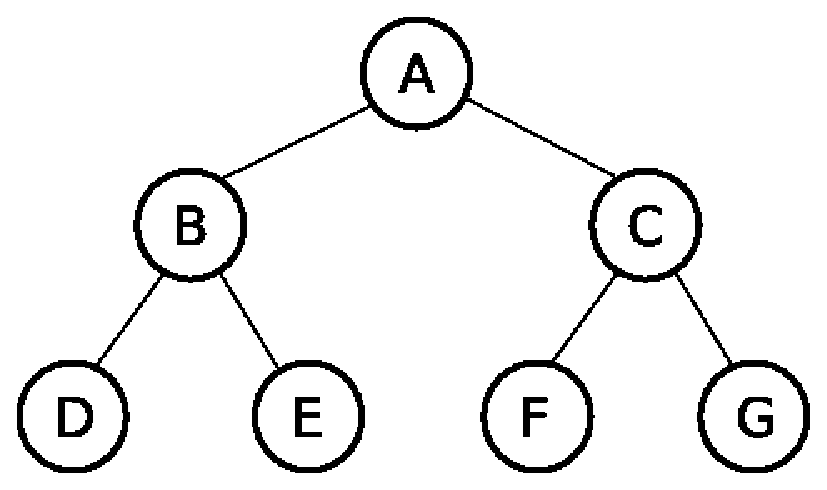
\includegraphics[scale=0.33]{binary_graph.eps}
  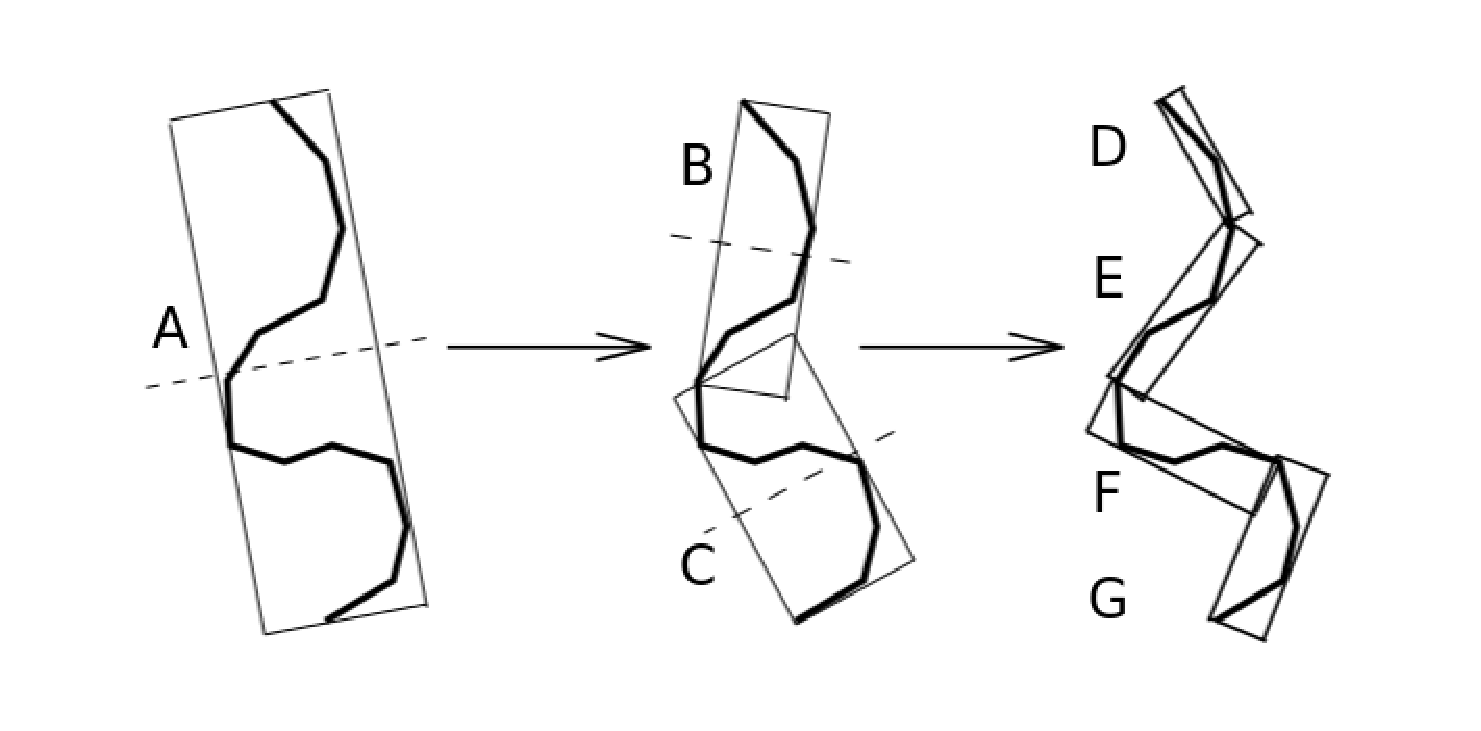
\includegraphics[scale=0.33, trim = 0 50 0 0 ]{bvh_2d_ex.eps}
  \caption[A 2D bounding volume hierarchy example.]{Depiction of a two dimensional BVH example adapted from Gottschalk 1996 \cite{Gottschalk_1996}}
  \label{fig:2D_bvh}
\end{figure}

In Weghorst's exploration of sphere and box bounding volumes it was found that
while spherical bounding volumes are not as computationally expensive to check
for ray intersections compared to bounding boxes, the latter generally provide a
tighter fit to the objects they contain. This decreases the chance of wasted
ray-volume intersection checks for rays which intersect the bounding volume but
not the object it contains. When considering the application of bounding volumes
to a discretized analytic surface represented by a triangle mesh, this becomes
more important as BVHs become deeper and more ray-volume intersection checks are
performed to reach leaf nodes. Even applied to analytic objects, this effect was
reflected in the results of Weghorts's work strongly enough to show that
bounding boxes provided better performance in accelerating the ray intersection
process than bounding spheres.

Two forms of BVHs are commonly applied in ray tracing problems: Axis-Aligned
Bounding Boxes (AABBs) and Oriented Bounding Boxes (OBBs). AABBs are boxes whose
orientation is restricted such that their faces are parallel to the problem's
global coordinate axes. Given a set of points to contain, aligned boxes are
straightforward to construct. Their simple representation results in a
relatively low memory footprint and computationally inexpensive ray-intersection
tests. Unlike AABBs, the axes of OBBs are allowed take any orientation relative
to the global axes in order to enclose their set of primitives as tightly as
possible. Due to the freedom in orientation, OBBs are able to bound sets of
primitives at least as tightly as AABBs, resulting in fewer unnecessary
intersection checks during the hierarchy traversal. Several robust methods for
determining the orientation of a box for best fit to a set of primitives have
been developed \cite{Gottschalk_1996,ORourke_1985}. OBBs are better for avoiding
superfluous ray-box intersections that might otherwise occur for an AABB. They
also more quickly conform to the full set of enclosed primitives as the boxes
are recursively divided. By orienting their axes with the local set of
primitives they are bounding, candidate splitting planes, usually selected in
the reference frame of the parent node's oriented axes, are more effective at
separating primitive entities and reaching leaf conditions quickly. This leads
to more shallow hierarchies making the worst-case number of intersection tests
lower than for an AABB hierarchy on average. While a shallow hierarchy might
indicate a smaller memory footprint, OBBs require one to store some extra
information about their orientation relative to the global axes making this
assumption difficult to prove consistently.

One disadvantage of using OBBs is that the ray-box intersection check requires
an extra step in transformation of the ray to the oriented axes of the box in
question at each level of the hierarchy traversal. The information needed for
transformation of the ray basis must be applied to the ray before the box
intersection can continue as it would for an axis aligned box. Thus, for a given
ray query, an OBB hierarchy may have fewer intersection checks to perform than
an AABB hierarchy, but the intersection checks are inherently more expensive
than in the case of OBBs. In practice, AABBs are commonly used in BVHs for their
simplicity of implementation and well-researched ray intersection
algorithms. Other reasons for this preference will be discussed later in Section
\ref{subsec:arch}.

There are multiple approaches to constructing a BVH around a set
of geometric primitives, but only ``top-down'' approaches will be discussed
here. A top-down approach begins with the construction of a single bounding
volume enclosing all primitives which will be part of the tree. At this point,
child boxes of this root node are created by selecting a splitting plane for
the box which divides the primitives contained by the current bounding volume
into two subsets. This process is then repeated until leaf conditions are
met. The selection of candidate splitting planes and the selection of a final
plane for splitting based on its estimated worth can greatly affect the
performance of the data structure.

One difficulty that BVHs face is that of overlapping sibling bounding
volumes. Overlapping sibling volumes can cause additional box intersection
checks in a similar manner to loosely fitting bounding volumes. If a ray passes
through a region of overlapping sibling volumes, this causes the children of
both boxes to be checked despite the fact that the desired nearest intersection
will be found in only one of those boxes. Overlaps are difficult to avoid,
however, due to the reality that volumes are required to contain discrete
elements, not just a section of the virtual space. Simply put, if
the splitting plane of a bounding volume goes through one of the geometric
primitives, there will be an overlap in the resulting child bounding
volumes. Overlaps of sibling AABBs are typically limited to the size of perhaps
one or two geometric primitives whereas overlaps between sibling OBBs are more
difficult to characterize as they may overlap regardless of the splitting plane
used. This inefficient characteristic of BVHs can be exacerbated by the
structure of triangulated objects the BVHs are being formed around. One such
feature which will be addressed in Chapter \ref{ch:high_valence}.

The spatial BVH variant (SBVH) was introduced by Stich et. al. in 2009
\cite{Stich_2009} with an additional complexity to the node splitting step. As
candidate split planes are considered, triangles (or geometric primitives) are
duplicated and contained in both resulting nodes. As a result, box boundaries do
not need to be re-calculated. They can be created directly by dividing the
parent bounding volume using the selected splitting plane. If a ray incident on
one of the duplicated primitives misses one of the boxes, the sibling box will
be intersected and the correct primitive intersection location will still be
found. This method grants much more freedom when considering how a node should
be partitioned. The relatively simple application of this method is performed by
considering both splits in which triangle duplication is prohibited and splits
in which it is allowed. In the scenario for which triangle duplication is
prohibited, the set of candidate planes is equivalent to that of a standard BVH
building algorithm. In the case where reference duplication is allowed, the
search for a splitting plane is much more open - as previously mentioned. In
fact, the search becomes closely aligned with the search for a spatial split as
might be found in KD-Tree construction. The optimal splitting plane is then
selected via a comparison of the cost for all candidate split planes - spatial
or ``traditional''. Secondary heuristics are used to limit reference splitting
in an effort to manage the data structure's memory footprint. The result of the
SBVH is a hierarchy which can be traversed just like any other BVH but with
significantly reduced sibling volume overlaps. The SBVH results consistently
show significant improvement over other methods \cite{Stich_2009}.

In summary, bounding volume hierarchies are favored in the field of ray tracing
for their relatively low memory footprints and well-developed parallel building
schemes while providing high performance ray tracing capabilities. These
features are of great import for systems with limited memory, such as GPUs, and
applications with intent for real-time viewing or interaction. These data
structures are particularly performant for \textit{Next Surface} intersections
and are currently the most commonly employed acceleration data structure for ray
tracing. They are relatively simple to implement for the performance they
provide and have smaller memory footprints relative to other ray tracing
acceleration data structures, making them attractive to memory-limited
environments such as GPUs.

\subsection{Octrees}%%Status:Done%%
\label{subsec:octree}

Octrees are a partitioning scheme in which cuboid bounding boxes, also
known as voxels, are used to partition the 3D problem space into eight
octants defined by the global axes and extents of the parent voxel. These eight
voxels are then linked as children of the parent voxel. This process is repeated
recursively until leaf conditions are met in which a sufficiently small number
of primitives is contained within the current voxel. This spatial subdivision
technique is commonly used to efficiently index data in 3-D space
\cite{Glassner_1989}. Octrees are somewhat like KD-trees in that their divisions
are purely spatial, their partitions contain no overlaps, and the placement of entities
in nodes occurs in a similar manner to that of KD-trees, but each node is
represented by a closed bounding volume as in a BVH.

Octrees can consume a large amount of memory relative to the data structures
previously discussed in this chapter. It is often possible that voxels may be
completely devoid of underlying entities. There are typically many voxels
containing no primitive references but may be required to exist as part of the
data structure, depending on its design. This results in many voxels being
stored in memory which aren't useful other than to verify that the space they
contain is empty. Additionally, geometric primitives may be referenced multiple
times if they intersect multiple nodes thus increasing the required memory
storage with the same consequence as seen in KD-Tree traversal with the
possibility of a primitive being checked more than once upon traversal. The
memory footprint is mostly of concern in applications for visualization on GPUs
- though specialized methods for octree applications on these architectures do
exist.

\begin{figure}[H]
  \centering
  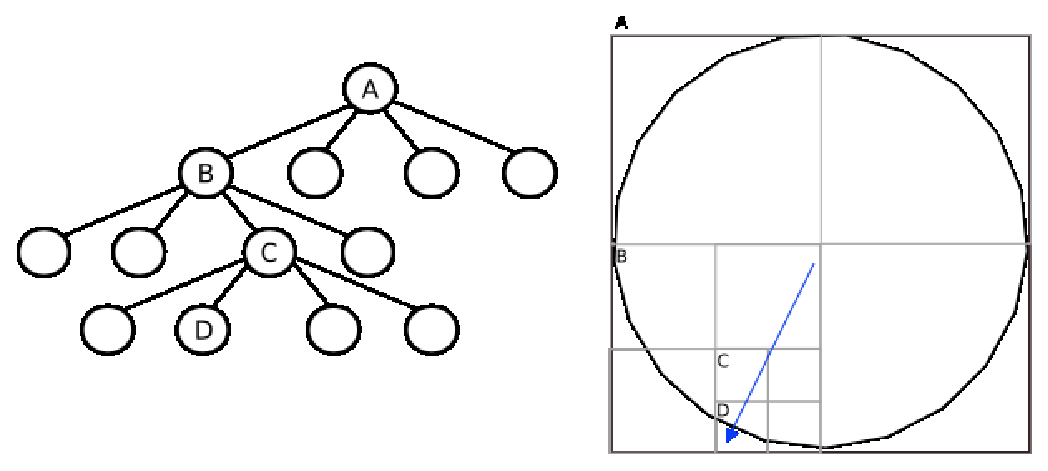
\includegraphics[scale=0.7]{octree_2d_ex.eps}
  \caption[A 2D octree example.]{Depiction of a two dimensional octree example of a top-down ray fire traversal for a simple geometric object.}
  \label{fig:2D_octree}
\end{figure}

One advantage of octrees is the regular nature of the partitions. The value of a
node in hierarchies such as these (or in the BVH for that matter) lies in its
ability to remove candidate space from the query, yet a voxel can only
accomplish this if rays strike the voxel. The result is that one measure of a
voxel's value can be described by the ratio of its probability of an
intersection check to the space it will exclude from the query search,
represented by its volume. In a problem with a uniform ray distribution, the
probability of a ray to intersect a given voxel can be related to a voxel's
surface area as seen in the SAH. Thus cubic voxels have the most favorable ratio
possible based on their geometry. The uniformity of voxel properties provide a
predictable nature of the octree which is advantageous when traversing the data
structure as well.

The predictable size and location of any given node in the tree determined from
the root node properties also provides a fast look-up of the deepest node in the
tree containing a point in space. This is helpful in providing a starting point
for ray traversal which is deeper than the root node, allowing one to
potentially avoid some traversal steps in the shallow levels of the
tree. Additionally, octrees have non-overlapping nodes which allows for
efficient traversal schemes similar to the neighbor linked traversal done in
KD-trees. These traversals are conceptually similar to that of the KD-tree's but
typically employ some form of Morton encoding to determine which node in the
octree the ray should visit next \cite{Revelles_2000}. Other traversal
techniques allow the octree to avoid creating and traversing nodes containing
empty space which can significantly reduce its memory footprint in cases where
internal nodes of the tree aren't required to define some spatial dataset as
mentioned above \cite{Samet_1989}. These methods are often applied in GPU
environments due to the limited memory available there. Octrees are often used
to store spatial data fields as well and naturally provide a higher resolution
of the field near boundaries of volume as the voxels become smaller in that
region which can be seen in Figure \ref{fig:2D_octree}.

As mentioned above, octrees are known for having large memory footprints
compared to other acceleration data structures, but they can also be used
advantageously for a combined purpose if a problem requires the storage of one
or more well-resolved data fields near volume boundaries as well as the
capability for ray tracing.

\subsection{Architecture-Based Acceleration}%%Status: Pending%%
\label{subsec:arch}

This section focuses on the impact of CPU architecture evolution on ray tracing
data structure design and implementation. More specifically, it emphasizes the
advantages of using vectorization-oriented implementations or Single Instruction
Multiple Data (SIMD) programming in the field of ray tracing.

When considering the problem of parallelism in computing, programmers focus on
one of two areas: \textit{functional parallelism} or \textit{data
  parallelism}. Functional parallelism describes the method of performing
multiple operations in parallel on many processors while data parallelism
describes operation on multiple data sets at the same time on a single
processor. SIMD is a form of data parallelism in which, as the name indicates,
the same set of numerical operations are performed on multiple sets of data in
parallel under a single CPU process. Chip-sets with support for SIMD
instructions became very popular in the mid-1990s as home PCs became more common
and demand for multimedia-related performance increased. In response, many CPU
manufacturers at the time such as Intel, IBM, and Motorola began to release
products with SIMD instruction sets, the most powerful of which was Intel's
Streaming SIMD Extensions (SSE). Over time, CPU clock speed became the larger
focus of many manufacturers as dramatic gains in processor speed took precedence
in the field. As processor speed increases began to wane, pushing the limit of
current cooling technology in the early 2000's, a new shift toward multi-core
designs occurred. Currently, as CPU clock speeds remain somewhat steady in
multi-core systems, a focus on single-thread performance via SIMD has
reemerged. Newer SIMD instruction sets such as Intel's Advanced Vector
Extensions (AVX or AVX2) have doubled the width of operable data, allowing for a
theoretical doubling of performance in codes relying on SIMD instructions
\cite{Hughes_2015}.

SIMD execution has found use in many different areas including medical imaging,
financial analysis, database management, computer visualization, and physical
simulation. As is the case in any problem well-suited to parallel programming,
all of these applications perform the same set of computations many times on
similarly structured sets of data. This situation arises quite often in
applications related to modeling or and visualization of virtual space. One
indicator of a problem which would benefit from parallel programming is the
presence of a few common sets of operations done many times or in a recursive
manner. Thus, traversal of ray tracing data structures is well suited for SIMD
operations as it relies heavily on the performance of a few key operations:
ray-node intersections and ray-primitive intersections. The ability to perform
intersection checks of many nodes at once or many triangles at once has clear
benefit when satisfying geometric queries in simulations or renderings which may
require several billion such operations. Several demonstrations of ray-tracing data
structures adapted to take advantage of SIMD-enabled optimization on modern CPUs
have already been developed.

\begin{figure}
  \centering
  \includegraphics[scale=0.6]{simd_ex.eps}
  \caption[Graphic representation of SIMD operations in CPUs.]{Concept of data parallelism using SIMD. Adapted from Intel's
    documentation on the advanced vector extensions (AVX) instruction
    set. \cite{Intel_AVX}}
  \label{fig:simd}
\end{figure}

An early implementation of SIMD used to intersect a ray with many triangles at
the leaf nodes of a KD-Tree was performed by Hurley in 2002
\cite{Hurley_2002}. This implementation demonstrated a significant improvement
in ray-primitive intersection performance and established many significant
observations about the utilization of SIMD commands within ray tracing
applications. Despite the fact that the cost of primitive intersection checks
was reduced, most of the time spent satisfying the ray query was spent in
traversal of the hierarchy to the leaf nodes. This is true of a well-formed BVH
and is verified for DAGMC in Figure \ref{dagmc-fng-coarse}. Noting that the
number of triangles in the KD-Tree's leaf nodes were small in comparison to the
SIMD registry width, Hurley described two ways in which to further exploit data
parallelism of SIMD in ray tracing.

One method is to traverse and intersect multiple rays at the same time. This is
refereed to as the N:1 approach. The other is to intersect many nodes with a
single ray which is referred to as the 1:N approach. An important characteristic
for success of the former method is that the group of rays being intersected has
very similar traversal paths through the hierarchy so they may be grouped
together in a packet for a narrow traversal path. This property is known as
often described as ray coherence. Branching off of Hurley's work, Wald
demonstrated that rays can be effectively grouped into packets and traversed in
a binary space partitioning tree (a modified KD-Tree) to achieve CPU performance
equal to that the high-end graphics hardware of the time \cite{Wald_2001}.

As more realistic physical effects are being applied in rendering applications
today (such as light-scattering surfaces, smoke effects, or fog), rendering ray
paths become less coherent. This means that the same primary rays will not
necessarily follow similar paths through the model or its underlying
acceleration hierarchies. Due to this lack of ray coherency, the 1:N approach to
data parallelism in which one ray is intersected with many hierarchy elements in
a single step has been revisited. Wald wisely observed that taking advantage of
SIMD operations in traversal of a KD-Tree is difficult due to the nature of the
partition. He goes on to state that the KD-Tree's superior serial performance in
comparison to that of serial BVH implementations drove reluctance to move away
from the KD-Tree and resulted in the establishment of ray packets, or
the 1:N approach \cite{Wald_2008}. Both Wald and Dammertz \cite{Dammertz_2008},
concurrently presented implementations of SIMD enabled traversal and primitive
intersection on multi-branching BVHs in 2008 with N:1 approaches. Both
implementations showed impressive performance enhancements, ranging anywhere
from 3-10 times faster than the baseline ray tracing kernels used for
comparison.

Both Wald and Dammertz approached the construction of multi-branching BVHs in
the same manner. Each built a standard binary BVH using the adjusted SAH cost
analysis in Figure \ref{adjusted_SAH} with median plane splitting. They then
collapsed the tree by directing child nodes to their ancestors to achieve the
desired branching ratio. Wald opted to use a more exotic, graphics-oriented,
architecture with Intel's Larrabee and was able to apply a branching ratio of 16
to their BVH while Dammertz used a branching ratio of 4 using Intel's Streaming
SIMD Extensions (SSE). A higher branching ratio provides higher SIMD utilization
and more shallow hierarchies, but Wald conceded that for common CPU-architectures
branching ratios between 4 and 8 would be optimal for most common architectures.

\begin{figure}
  \begin{center}
    \includegraphics[scale=0.25]{obb-conformity.eps}
  \end{center}
  \caption[Graphic of bounding volumes surrounding a torus.]{A figure replicated
    from Gottschalk's paper on OBBs exemplifying OBB's rapid conformity to a
    torus volume (right) in comparison to AABBS (left).}
  \label{fig:obb-conformity}
\end{figure}

AABBs were used in both Wald and Dammertz's implementations. While OBBs have
been shown to conform more quickly to the underlying geometry and can generate
more shallow trees as seen in Figure \ref{fig:obb-conformity} , AABBs are
generally more favorable in SIMD implementations. First, OBBs require more
information to be stored. This extra information can limit how many nodes will
fit into a single SIMD step and it is often more beneficial to check more AABBs
than fewer OBBs despite the tighter fitting to geometric primitives. This is in
part because AABBs boxes have faster ray intersection tests without the
re-orientation of the ray information to the box coordinates, but also because
more nodes can be fit into the SIMD register to be visited at once. Secondly,
though OBB hierarchies are more shallow than their axis aligned counterparts',
tree depth is of less concern due to the higher n-ary structure of the trees
used in these implementations.

\setcounter{footnote}{1}

\begin{figure}[H]
  \begin{equation}
    C = C_t + \sum_{k=0}^{K} \frac{SA(B_k)}{SA(B)}\frac{|P_k|}{T}C_i
  \end{equation}
  \begin{align*}
    K - & \, number \, of \, desired \, children \, per \, interior \, node \\
    T - & \, number \, of \, triangles \, in \, SIMD \, register
  \end{align*}
  \caption[Form of the surface area heuristic for an n-ary tree.]{An adjusted
    form of the surface area heuristic for an n-ary BVH branching ratio as
    presented by Wald in \cite{Wald_2008}. \protect\footnotemark}
  \label{adjusted_SAH}
\end{figure}

\footnotetext{Some notation has been modified to agree with
  notation used in Figure \ref{fig:SAH}}

% NOT SURE THIS IS NECESSARY %
For completeness of all ray tracing data structures discussed in this chapter,
SIMD implementations of octrees were sought out in literature, but none were
found. This is likely due to the fact that SIMD registers on common
architectures wide enough to accommodate 8 nodes are not yet common. It is also
worth noting that while the KD-Tree is restricted to a binary hierarchy, another
variation, the bounding interval hierarchy, might be compatible with higher
branching ratios and thus SIMD traversal of the hierarchy \cite{Watcher_2006}.

\subsubsection{Application in Embree}

Many of these concepts have been applied in a ray tracing kernel called Embree.
Embree is the result of an effort to produce a performant CPU-based ray tracer
as a demonstration of the expanding capabilities of modern CPU architectures
\cite{Wald_2014}. In both construction and traversal of its BVHs, Embree takes
advantage of many of the latest developments in BVH research and using modern
chipset architecture capabilities via vectorization at an implementation level.
The combination of these effects leads to a very powerful ray tracing tool in
terms of performance, as demonstrated by the many projects which have
incorporated Embree as their production ray tracing kernel such as Corona,
Autodesk, FluidRay, and Brighter3D. As a result of its success in other areas,
Embree was selected for application in DAGMC to satisfy geometric queries for
attached physics kernels. Several critial design features of Embree will be
reviewed here and their importance to efficient BVH traversal discussed.

\paragraph{Memory Alignment}

For the CPU architectures used in this work, Embree's quad-tree implementation
was applied. In order to use this design in a SIMD context, the code constructs
must be carefully designed for interpretation by the CPU. Embree defines
BVH-related structures such that they occupy aligned memory spaces, meaning that
they are both compact in memory usage and can be read into CPU registers in
a predictible manner. All bounding volumes and the underlying Cartesian vector
types used to define them are specified as structures aligned to 16 bytes in
memory. This is important for encoding of node types and leaf sizes, discussed
in Section \ref{sec:node_encoding}, as well as the ability for these types to be
operated on as either arrays of floats during BVH construction or as native SIMD
types during BVH traversal.

\paragraph{Node Type Encoding}\label{sec:node_encoding}

Nodes in Embree's BVH are stored compactly using an encoding scheme which contains
the memory address of box information as an integer value. Because nodes are
byte-aligned, memory addresses will be offset by the same amount as the node
alignment. For example, if nodes are memory aligned to 16 bytes, the four least
significant bits in the integer representations will be unused. These bits are
used to encode information about both leaf nodes and empty nodes. Empty nodes
required as part of the data structure but don't contain primitive entities. Figure
\ref{fig:node_encoding} depicts the bits of a leaf node for reference.

\begin{figure}[H]
  \centering
  \includesvg{../images/node_encoding}{width=1.0\textwidth}
  \caption[Graphic of leaf node encoding.]{Visual representation of leaf
    encoding using integer-based pointer values. \textcolor{Dandelion}{Yellow}
    digits represent bits used to store the address of the first primitive
    reference in the tree. The \textcolor{BrickRed}{red} digit indicates the fourth least significant
    digit which is used to indicate that the stored memory address points to a
    primitive reference rather than another node reference. The final three
    \textcolor{ForestGreen}{green} digits indicate the number of primitive references in the leaf node.}
  \label{fig:node_encoding}
\end{figure}

This representation reduces memory storage of leaf nodes, which can be
considerable given that the number of leaf nodes in a n-ary tree is

\begin{equation}
 L = n^{h}
\end{equation}

\begin{align*}
   L - & \textrm{number of leaf nodes in the tree} \\
   n - & \, \textrm{n-ary  of  the  tree  (branching  ratio)} \\
   h - &  \textrm{height  of  the  tree  (zero-indexed)} \\
\end{align*}

meaning a quad tree with a height of ten will contain over one million leaf
nodes. Avoiding storage of the memory address and leaf node size separately
reduces memory consumption of the tree and allows the use of fast bit-wise
operations to differentiate node types when traversing the tree.

\paragraph{Memory Prefetching}

While CPU clock speeds are getting faster each generation, memory latency is
often the limiting factor in the performance of many algorithms (see Figure
\ref{fig:memory_latency}). To account for this latency, modern CPUs allow
compilers and code writers to initiate asynchronous requests for memory access
before it's needed for computation. This technique, known as memory prefetching, avoids memory
latency by populating low level memory caches with data before it is required by
the CPU.

\begin{figure}[H]
\centering
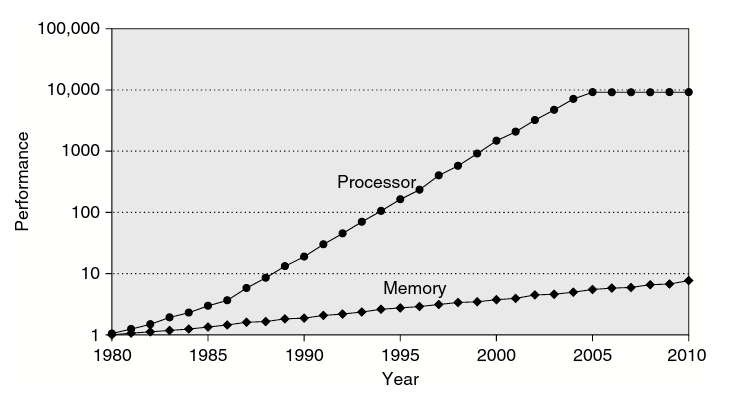
\includegraphics[width=0.9\textwidth]{../images/mem_latency.png}
\caption[Memory latency comparison over time.]{Trends in CPU vs. memory
  performance over time. The processor line shows the increase in memory
  requests per second on average. The memory line shows the increase in memory
  accesses per second. \cite{Hennessy_2012}}
\label{fig:memory_latency}
\end{figure}

Memory prefetching is applied automatically by compilers in situations where the
compiler can clearly determine the next blocks of memory needed by the
CPU. Several common patterns are used by compilers to predict memory access
including \textbf{Next-Line} and \textbf{Next-N-Line} prefetching. These
patterns are often applied when looping over large arrays of data. Next-Line
prefetching gathers information for the next iteration of the loop during the
current iteration. Next-N-Line prefetching groups the loop iterations together
to improve the timing between prefetching and computation for the CPU. Proper timing
prefetch operations is critical. Memory fetched too early may bump information
out of the CPU cache still needed by the current iteration's computational
block, causing additional memory latency to re-gather that data. Memory fetched
too late defeats the purpose of applying prefetching and can interfere with
automatic memory access requests from the CPU. Examples of both Next-Line and
Next-N-Line prefetching can be seen in \ref{fig:prefetch_examples}. Modern
compilers are becoming increasingly adept at predicting memory access for these
cases and will apply prefetching as part of resulting instruction sets.

\begin{figure}[H]
  \begin{subfigure}[t]{0.48\textwidth}
    \centering
    \includesvg{../images/next-line_prefetch}{width=\textwidth}
    \caption{Next-Line Prefetching}
    \vfill
  \end{subfigure}
  \hfill
  \begin{subfigure}[t]{0.48\textwidth}
    \centering
    \includesvg{../images/next-n-line_prefetch}{width=\textwidth}
    \caption{Next-N-Line Prefetching.}
  \end{subfigure}
  \caption[Compiler memory prefetching examples.]{Example of manually implemented
    memory prefetching for a standard loop performing a vector operation. This
    type of pattern is often automatically implemented by modern compilers.}
  \label{fig:prefetch_examples}
\end{figure}

Memory prefetching can also be applied manually in situations where the user is
aware of the next memory block to be used by the CPU as well. One example of a
user-informed prefetching method is \textbf{Pointer-Based} prefetching. In this method,
memory locations pointed to by locally accessed data structures are known to be
operated on soon by the CPU are prefetched. This method is commonly applied when
traversing hierarchical data structures or linked lists. An example of
Pointer-Based prefetching can be found in \ref{fig:pointer_prefetching}. The
traversal of the BVH in Embree takes advantage of this particular prefetching
pattern to reduce memory latency. Because of the indirection involved in
traversal of data structures by pointer and the result-based operations at each
node in the structure, it is very difficult for compilers to predict memory
access patterns and apply prefetching automatically. Application of these
Pointer-Based methods are nearly always applied manually.

\begin{figure}[H]
\centering
\includesvg{../images/pointer_prefetch}{width=0.45\textwidth}
\caption[Manual memory prefetching example.]{Example of a prefetch pattern using
  pointers to follow a data structure traversal.}
\label{fig:pointer_prefetching}
\end{figure}

Embree applies Pointer-Based prefetching while traversing its BVH. As nodes
intersected by the ray are added to the stack, the bounding box
information for the node at the top of the stack is prefetched for intersection
in the next step of the BVH traversal.

\paragraph{Ray-Box Intersection Tests}

In order to take advantage of compiler optimization and SIMD instructions,
ray-box tests in Embree contain a no branching (no if-else statements) version of
Kay's slab box intersection test \cite{Kay_1986}. Removing branching avoids
additional memory fetching or re-organizing of CPU registers so that SIMD
operations can be efficiently performed in sequence to determine intersection
locations with the box along each dimension. Underlying SIMD computation
calculates the intersection of a ray with several boxes at once without memory
disruption. The distances to intersection along the ray for each box coordinate
are then compared to find the near and far intersections with axis-aligned
bounding box planes. If the largest of the near-side intersections is smaller
than the smallest of the far-side intersections, then the ray strikes the box.

To perform this computation efficiently, some information is pre-computed and
added to the ray structure including the inverse of the ray direction. These
values are also duplicated into memory-aligned vector types with sizes equal to
the n-ary of the BVH, again so that memory doesn't need to be allocated
on-the-fly during traversal of the data structure. A bit-mask is used to
indicate which boxes are hit and which are not, and the distance to each box
intersection is returned so that the closest boxes can be added at the top of
the traversal stack.

%% \begin{lstlisting}[language=Python,basicstyle=\tiny,caption={A non-branching ray-node intersection test for a quad tree implementation.},
%%     label={alg:no-branch ray-box pseudo code},captionpos=b]

%%   def ray_node_intersection(ray, node):
%%       # result - mask (0 - miss, 1 - hit)
%%       # inverse direction - ray.invdir
%%       # inverse direction times the ray origin - ray.org_invdir
%%       # tNear/tFar - parameter value of intersections along ray direction

%%       # compute tNear for N nodes
%%       tLowerX = node.lowerX * ray.invdir.x - ray.org.x * ray.invdir.x
%%       tLowerY = node.lowerY * ray.invdir.y - ray.org.y * ray.invdir.y
%%       tLowerZ = node.lowerZ * ray.invdir.z - ray.org.z * ray.invdir.z

%%       # compute tFar for N nodes
%%       tUpperX = node.upperX * ray.invdir.x - ray.org.x * ray.invdir.x
%%       tUpperY = node.upperY * ray.invdir.y - ray.org.y * ray.invdir.y
%%       tUpperZ = node.upperZ * ray.invdir.z - ray.org.z * ray.invdir.z

%%       # determine near/far values
%%       tNearX = min(tLowerX, tUpperX)
%%       tNearY = min(tLowerY, tUpperY)
%%       tNearZ = min(tLowerZ, tUpperZ)
%%       tFarX =  max(tLowerX, tUpperX)
%%       tFarY =  max(tLowerY, tUpperY)
%%       tFarZ =  max(tLowerZ, tUpperZ)

%%       # compute maximum tnear for all boxes
%%       tNear = max(tNearX, tNearY, tNearZ, ray.tNear)
%%       tFar =  min(tFarX,  tFarY,  tFarZ,  ray.tFar )

%%       # compute a mask indicating which boxes are hit
%%       mask = tNear <= tFar

%%       # set distances to intersection to optimize traversal (nearest nodes first)
%%       dist = tNear

%%       return mask, dist
%% \end{lstlisting}

\begin{lstlisting}[language=Python,basicstyle=\tiny,caption={A non-branching
      ray-node intersection test for a quad tree implementation with pre-computed
      near and far box coordinate values.},
    label={alg:no-branch ray-box optimized},captionpos=b]

  def ray_node_intersection(ray, node):
      # result - mask (0 - miss, 1 - hit)
      # inverse direction - ray.invdir
      # inverse direction times the ray origin - ray.org_invdir
      # tNear/tFar - parameter value of intersections along ray direction

      # compute tNear for N nodes
      tNearX = vecN(&node + ray.nearX) * ray.invdir.x - ray.org.x * ray.invdir.x
      tNearY = vecN(&node + ray.nearY) * ray.invdir.y - ray.org.y * ray.invdir.y
      tNearZ = vecN(&node + ray.nearZ) * ray.invdir.z - ray.org.z * ray.invdir.z

      # compute tFar for N nodes
      tFarX = vecN(&node + ray.farX) * ray.invdir.x - ray.org.x * ray.invdir.x
      tFarY = vecN(&node + ray.farY) * ray.invdir.y - ray.org.y * ray.invdir.y
      tFarZ = vecN(&node + ray.farZ) * ray.invdir.z - ray.org.z * ray.invdir.z

      # compute maximum tnear for all boxes
      tNear = max(tNearX, tNearY, tNearZ, ray.tNear)
      tFar =  min(tFarX,  tFarY,  tFarZ,  ray.tFar )

      # compute a mask indicating which boxes are hit
      mask = tNear <= tFar

      # set distances to intersection to optimize traversal (nearest nodes first)
      dist = tNear

      return mask, dist
\end{lstlisting}


Further optimization is accomplished by pre-computing the near and far side
coordinates based on the signs of the ray's unit direction. In this way, the
near and far coordinates of the box are already known. Thus the near and far
intersections do not require sorting along each box axis and cand be directly
computed. To avoid branching and structure indexing in the ray-box intersection
computation, byte offsets values are pre-set on the ray. These offset values are
used during intersection tests to gather the correct coordinate values for the
child boxes of a node in the hierarchy rather checking Boolean values and adding
branches to the test. After computing the near and far side intersections, the
maximum near-side and minimum far-side hit distances still need to be found, but
skipping the comparison of values for each axis removes a considerable portion
of computation from the test. An example of this method is shown in Figure
\ref{alg:no-branch ray-box optimized}. It is worth noting that this optimization
is not applicable when using OBBs. The unknown orientation of the box axes makes any
prediction about which side of the box will be intersected first by the ray
impossible. In this case the ray-box intersection must include an additional
step to sort the near and far side hits before checking for intersection.

\subsection{Signed Distance Fields}

Signed Distance Fields (SDFs) are commonly derived from implicit surface
functions and variations on these functions are known as level-set functions
\cite{Osher_2003}. Both offer a rich and versatile representation of closed
manifolds used for modeling, simulation, and rendering. As discussed in Section
\ref{subsec:implicit_surfaces}, Constructive Solid Geometry (CSG)
representations seen in native Monte Carlo codes are formed from Boolean
combinations of predefined implicit surfaces at their core. While these
predefined surfaces do not give the freedom of model creation and manipulation
found in many CAD systems, important geometric information required for
visualization and simulation can be readily recovered from implicit surfaces.

\begin{figure}[H]
  \includesvg{../images/preconditioner_datastruct}{width=0.5\textwidth}
  \centering
  \caption[2D depiction of a signed distance field.]{2D visualization of a signed distance field surrounding an arbitrary volume boundary.}
  \label{fig:preconditioner_datastruct}
\end{figure}


%% Implicit surface functions are multivariate functions defined over the
%% $R^3$ domain as:
%% \begin{equation} \label{eq:implicit_surf_rep}
%%       \Omega(R^3)\rightarrow R
%% \end{equation}
%% where an isocontour of value, $v$, of the implicit surface can be
%% described as
%% \begin{equation} \label{eq:implicit_surf_isocontour}
%%   \Omega(\vec{x}) - v  = 0
%% \end{equation}
%% for all points $\vec{x}$ satisfying that equation. For simplicity, the surface
%% isocontour value is typically defined as $0$.

%% By recognizing that the magnitude of $\Omega(\vec{x})$ is in fact a
%% minimum interface distance function, one can construct a signed
%% distance function, $SDV(\vec{x})$, using the isocontour representation
%% and the magnitude of the function as seen in Eq.~\eqref{eq:sdf}
%% \cite{Osher_2003}.

%% \begin{align} \label{eq:sdf}
%%    SDV(\vec{x}) = |\Omega(\vec{x})|
%% \end{align}

Signed distance field generation from implicit surfaces is a particularly
valuable property of this geometric representation. A signed distance field,
meets the following requirements for any vertex, $v$, in the
total set of locations, $V$, in the field:

\begin{itemize}
\item $ |SDF(v)| = min(|\vec{x}-\vec{x_I}|) \, \forall \, v \, \in \, V$
\item $ SDF(v) = 0 \, \forall \, v$ on the surface boundary
\item $ SDF(v) > 0 \, \forall \, v$ inside the surface boundary, and
\item $ SDF(v) < 0 \, \forall \, v$ outside the surface boundary
\end{itemize}

Implicit surfaces can be naturally extended to represent dynamic geometries by
including a time dependence in the function, making them powerful tools for
populating signed distance fields in simulation and rendering of fluids, smoke,
fire, etc. To simulate these phenomenon, the data structure is populated with
signed distance values for a given time in the rendering (see Figure
\ref{fig:preconditioner_datastruct}). The signed distance field can then be used
to determine point containment queries and approximate nearest surfaces
values. It can also trace rays at any time via a method in which the ray length
is repeatedly clipped using signed distance values to approach a surface in a
process called ray marching \cite{Tomczak_2012}.

\section{Monte Carlo Memory Considerations}\label{sec:mc_mem}

The bulk of Monte Carlo memory consumption in native calculations is attributed
to nuclear cross-section data and tally data structures with the analytic CSG
geometry representation taking up a small portion of the overall program memory.

\subsection{Cross-Section Data}

Cross-section data is necessary to represent the physical
processes governing particle transport through the virtual geometry. Various
formats of this data exist with both continuous and discrete representation of
cross section information.

Continuous representations of this data can occupy a considerable amount of
space and are more computationally expensive to evaluate than discrete
representations, but are also more accurate. Discrete representations of this
data consume more memory in simulation, but require less computation when
extracting data. The amount of memory occupied by nuclear data is dependent on
the number of unique materials used in the problem as well as the material
composition in terms of the unique isotopes in the problem. This data can occupy
the majority of simulation memory for large problems with many materials.

\subsection{Tally Data Structures}

Results of the Monte Carlo calculation are kept as tallies of particle
contributions to physical quantities at various locations in the physical
model. Tallies on surfaces or in cells change the memory usage of the simulation
insignificantly, unless additional data is needed to calculate derived
quantities. Mesh-based tallies on the other hand can dominate the memory
usage. In MCNP and many other Monte Carlo codes, mesh tallies are defined by the
user as structured grids in either Cartesian, cylindrical, or spherical
coordinates. These tallies are often used for better spatial resolution of
physical data in the simulation and for coupling to analysis in other
engineering domains. Tetrahedral mesh tallies are also supported by several
Monte Carlo codes DAGMC interacts with, including MCNP
\cite{LANL_MCNP5_VOLIII}. The size of these tallies vary based on the needs of
the user and the trade-offs associated with spatial resolution of solutions and
statistical convergence related to mesh element sizes.

\subsection{Impact on CAD-Based Tessellations}

For the Monte Carlo code used in this work, MCNP, the parallelism method applied
is a master/slave scheme standard for many applications using the Message
Passing Interface (MPI) \cite{Forum_1994}. The master process is responsible for
initializing the problem, determining the load balance for the number of
parallel processes requested by the user, and collecting/accumulating
information at the end of the simulation. In MCNP, particle histories are
divided into equal segments among the slave processes for evaluation. More
information on the method for particle history division and random number
sequence assignment was detailed by Deng and Xie \cite{Deng_1999}. For each
slave process, a corresponding set of the nuclear data, tally data structures,
and geometry representation are created. Duplication of the geometry
representation has a significant implications for the use of CAD-based
tessellations.

The tessellations resulting from CAD geometries consume much more memory than
corresponding CSG representations. This must be taken into consideration when
planning parallel simulations on clusters where the limitation for the number of
processes per CPU is often the memory used per process. Because DAGMC's
CAD-based particle tracking is an addition to MCNP, it has no influence on the
parallelism data model. Given that geometry representations are required to
exist in each process of the parallel simulation, memory usage in DAGMC is
closely monitored. Some of this memory usage is largely uncontrollable due to
the reliance on CUBIT or Trelis' underlying tessellation algorithms, but
additional data used to maintain geometric relationships and build acceleration
data structures are kept to a minimum if possible.

\begin{table}[H]
    \centering
  \begin{tabular}{l c c c}
    \toprule
    Model & Tessellation (MB) & Tessellation and MOAB BVH (MB) & Simulation (MB) \\
    \hline
    FNG   & 92           & 213  & 262  \\
    ATR   & 294          & 765  & 865  \\
    UWNR  & 213          & 446  & 1250 \\
    nTOF  & 56           &  88  & 416  \\
    ITER  & 2592         & 5547 & 6679 \\
    \hline
  \end{tabular}
  \caption[Memory summary of performance benchmark models.]{A summary of the
    memory usage for the performance benchmark models shown in Table
    \ref{dag-mcnp-benchmarks} both with and without acceleration data structures.}
  \label{tab:dag-mcnp-benchmarks-mem}
\end{table}

Table \ref{tab:dag-mcnp-benchmarks-mem} shows the memory usage for all of the
benchmark models used to assess DAG-MCNP's performance relative to native MCNP
geometry representations in Section \ref{sec:problem-statement}. All of the
models consume relatively low amounts of memory compared to the storage found on
many CPUs in High Performance Computing (HPC) environments, but the addition of
acceleration data structures, in this instance MOAB's BVH of OBBs, can more than
double the memory occupied for the geometry representation. This effect becomes
even more pronounced in larger production models seen in Chapters
\ref{ch:simd_bvh} and \ref{ch:high_valence}, though shared memory
implementations for higher per-node memory efficiency are on DAGMC's development
path.

In addition to the benchmark models from Table \ref{dag-mcnp-benchmarks}, Table
\ref{tab:dag-mcnp-benchmarks-mem} includes a model of a demonstration nuclear
fusion device currently under construction in southern France.  An analysis of
ITER using DAGMC was performed at the University of Wisconsin - Madison to
calculate a spatial mapping of the dose rate induced by irradiated components of
the machine for various cooling times or times after shutdown of the device.
This shutdown dose rate calculation was broken into seven spatial source meshes
to avoid exceeding the memory limits of the HPC cluster used for this
analysis. The values displayed in the table represent the memory usage for one
of the seven simulations required to complete the analysis. This model was
included as a current representation of the analysis work being performed in
DAGMC. It was not included in the comparative benchmark analysis of DAGMC
because no native MCNP counterpart of this model exists. This model contains
components created in CAD with no analogous MCNP representation, another reason
CAD-based tessellations are desirable for MCRT. The simulation memory footprint
of the ITER model is much larger in simulation, so much so that the number of
processes allocated to a node was memory-limited rather than core-limited during
analysis.

\section{Summary}

This discussion of the CAD-based MCRT-t via the DAGMC toolkit, hierarchical
spatial data structures, SDF generation, and context for memory use in parallel
simulations with MCNP in this chapter provides a basis for the work performed in
the remainder of this document. Chapter
\ref{ch:preconditioning} discusses the implementation and application of SDFs in
DAGMC's framework. Next, Chapter \ref{ch:simd_bvh} presents work on BVHs
optimized for use in DAGMC and extensions of those methods to provide robust
transport in production simulations. Chapter \ref{ch:high_valence} discusses the
effects of splitting heuristics and hierarchy construction surrounding
problematic geometric features on the performance of DAGMC simulations.
